\documentclass[10pt,twocolumn]{article}
\usepackage{times}
\usepackage{multirow}
\usepackage{tabularx}
\usepackage{caption}
\usepackage{subcaption}
\usepackage{graphicx,grffile}
\usepackage{pgf}
\usepackage{tikz}
\usepackage{listings}
\usepackage{color}
\usetikzlibrary{arrows,automata}
%\usepackage[latin1]{inputenc}

\definecolor{mygray}{rgb}{0.5,0.5,0.5}
\lstset{frame=tb,
  language=Ruby,
  basicstyle={\scriptsize\ttfamily},
  breaklines=true,
  captionpos=b,
  numbers=left,
  numbersep=5pt,
  numberstyle=\tiny\color{mygray},
  xleftmargin=2em,
frame=l,
framexleftmargin=1.5em
}

%  aboveskip=3mm,
%  belowskip=3mm,
%  showstringspaces=false,
%  %columns=flexible,
%  basicstyle={\scriptsize\ttfamily},
%  %numberstyle=\tiny\color{gray},
%  %keywordstyle=\color{blue},
%  %commentstyle=\color{dkgreen},
%  %stringstyle=\color{mauve},
%  %breaklines=true,
%  breakatwhitespace=true,
%  tabsize=3
%}

% do not change these values
\baselineskip 12pt
\textheight 9in
\textwidth 6.5in
\oddsidemargin 0in
\topmargin 0in
\headheight 0in
\headsep 0in

%\makeatletter
%\def\maxwidth{\ifdim\Gin@nat@width>\linewidth\linewidth\else\Gin@nat@width\fi}
%\def\maxheight{\ifdim\Gin@nat@height>\textheight\textheight\else\Gin@nat@height\fi}
%\makeatother
%% Scale images if necessary, so that they will not overflow the page
%% margins by default, and it is still possible to overwrite the defaults
%% using explicit options in \includegraphics[width, height, ...]{}
%\setkeys{Gin}{width=\maxwidth,height=\maxheight,keepaspectratio}
%

\usepackage[unicode=true]{hyperref}
\hypersetup{breaklinks=true,
            bookmarks=true,
            pdfauthor={},
            pdftitle={},
            colorlinks=true,
            citecolor=blue,
            urlcolor=blue,
            linkcolor=blue,
            pdfborder={0 0 0}}
\urlstyle{same}  % don't use monospace font for urls

\usepackage[font=footnotesize,labelfont=bf]{caption}

\begin{document}

\title{brados: declarative, programmable object storage}

\author{
Noah Watkins, Michael Sevilla, Ivo Jimenez, \\Neha Ojha, Peter Alvaro, Carlos
Maltzahn\\
\small {\em University of California, Santa Cruz} \\
%\small {\{jayhawk,carlosm\}@cs.ucsc.edu} \textsuperscript{*}nojha@ucsc.edu \\ [2mm]
\small Submission Type: Research
}

\date{}
\maketitle

\begin{abstract}
To meet the needs of a diverse and growing set of cloud-based applications,
modern distributed storage frameworks expose a variety of composable
subsystems as building blocks.  This approach gives infrastructure programmers
significant flexibility in implementing application-specific semantics while
reusing trusted components.  Unfortunately, in current storage systems the
composition of subsystems is a low-level task that couples (and hence
obscures) a variety of orthogonal concerns, including functional correctness
and performance.  Building an application by wiring together a collection of
components typically requires thousands of lines of carefully-written C++
code, an effort that must be repeated whenever device or subsystem
characteristics change.

In this paper, we propose a declarative approach to subservice composition
that allows programmers to focus on the high-level functional properties that
are required by applications.  Choosing an implementation that is consistent
with the declarative functional specification then can be posed as a search
problem over the space of parameters such as block sizes, storage interfaces
(e.g. key/value or block storage) and concurrency control mechanisms.  We
present experimental evaluation of our prototype, (etc etc)
\end{abstract}

\section{Introduction}

% whats the problem
Storage systems are increasingly providing features that take advantage of
application-specific knowledge to achieve optimizations and provide unique
services. However, this trend is leading to the creation of a large number of
software extensions that will be difficult to maintain as system software and
hardware continue to evolve.

%%% Anderson FAST 2016 IoT Time Series DB on Ceph

% why is it interesting
The standardization of the POSIX file I/O interface has been a major success,
allowing application developers to avoid vendor lock-in. However, large-scale
storage systems have been dominated by proprietary products, preventing
exploration of alternative interfaces and complicating future migration paths,
eliminating the benefits of commodity systems. But the recent availability of
high-performance open-source storage systems is changing the way people
approach storage because these
systems are modifiable, enabling interface change and reducing the risks of
lock-in. The widely deployed Ceph distributed storage system is an example of
a storage system that supports application-specific extensions in the form of
custom I/O interfaces to objects managed by the underlying RADOS object
storage system~\cite{weil:osdi06,weil:pdsw07}. Organizations are increasingly
reliant upon these extensions. Figure~\ref{fig:objclass-dev} shows
a marked increase in the number of object operations that are packaged as part
of the Ceph distribution and widely used by internal Ceph subsystems and by
applications such as OpenStack Swift and Cinder~\cite{openstack}.
Unfortunately, the code composing these interfaces
is written assuming a performance profile defined by the combination of the
hardware and software versions available at the time of development.

\begin{figure}[t]
  \centering
    \includegraphics[width=0.48\textwidth]{experiments/objclass-dev/output.png}
    \caption{
[\href{https://github.com/noahdesu/zlog-popper/tree/master/experiments/objclass-dev/visualize.ipynb}{source}]
Growth of officially supported, custom object interfaces in RADOS over 6
years. An \emph{operation} is a function executed in the context of an object,
and operations are grouped into different \emph{categories}
corresponding to applications or utilities, such as reference counting}
\label{fig:objclass-dev}
\end{figure}

%%% why is it hard / why do naive approaches fail
In addition to the growth in the quantity of operations in use throughout Ceph
installations, Figure~\ref{fig:objclass-dev} also depicts the amount of
low-level C++ written to implement these operations.
While
the bulk of these interfaces are created by core Ceph developers with a
complete view of the performance model, this may be changing. The
development community has been receptive to outside contributions with the
recent inclusion by CERN developers of an extension for performing limited
numeric operations on object data~\cite{cls_numops}. And while Ceph has not
yet reached the point of directly exposing these features to
non-administrative users, the inclusion of a mechanism for dynamically
defining extensions using Lua~\cite{cls_lua} (currently pending review)
suggests that aspects of this
feature may soon appear. What is needed is support for creating storage
interfaces using a method that allows transparent optimization as the system,
application, and supporting environment evolve.

% why hasn't it been solved before / why have previous approaches failed
Unfortunately the size of the design space for even simple interfaces can
be very large, and it can be difficult to choose a design that
``future-proofs'' an
implementation against hardware and software upgrades.
Previous work related to storage interface design has largely been in the
context of standardization efforts and active storage. While the former is
primarily concerned with fixed interfaces, application-specific interfaces
built using active storage techniques have not to the best of our knoweldge
addressed portability concerns that arise from defining interfaces
imperatively. We address this gap by using a declarative language we call
\emph{brados} to define application-specific storage interfaces in
object-based storage systems, decoupling interface definition from
implementation and allowing interfaces to adapt to system changes without
modification.

To demonstrate the use of the \emph{brados} language we will show how a
high-performance shared-log based on the CORFU protocol can be built in Ceph, as well
as existing real-world interfaces used in the Ceph storage system. First we
discuss the Ceph storage system which our prototype is built upon and the 
motivating system, CORFU. We then present the challenges that programmers face
when navigating the design space during the process of building an
application-storage interface. The \emph{brados} language is then described
using the CORFU system and an existing Ceph-specific interface as motivating examples.
We conclude by discussing the optimization opportunities that we can realize
using analysis of interfaces. We hope you enjoy the show.

\section{Background}

In this section we describe the salient components of Ceph that we use to
construct application-specific extensions, and provide an overview of the
CORFU distributed shared-log which is the primary motivating example used in
this paper. The content of this section sets the stage for a discussion of the
complexities developers face building application-specific storage interfaces.

\subsection{Ceph Basics and Storage Interfaces}
\label{sec:objclass}

Figure~\ref{fig:ceph} illustrates the collection of components commonly
referred to as Ceph. At the bottom, a cluster of 10s--10,000s of \emph{object
storage devices} compose the distributed object storage system called RADOS.
Widely deployed applications such as the S3/Swift--compliant RADOS Gateway
(RGW), RADOS Block Device (RBD), and the POSIX Ceph File System are built upon
the \emph{librados} client layer that presents a fault-tolerant always-on view
of the RADOS cluster.

\begin{figure}[t]
  \centering
  \begin{subfigure}[b]{.48\linewidth}
      \centering
      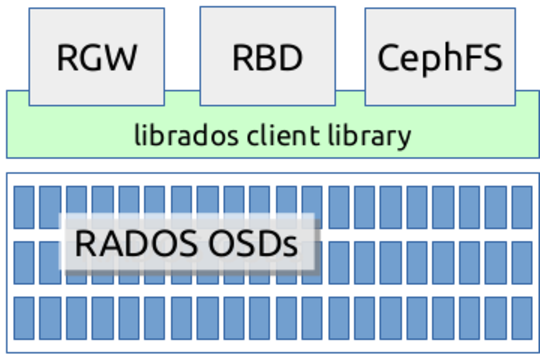
\includegraphics[width=1.0\linewidth]{figures/ceph}
      \caption{Ceph Cluster}
      \label{fig:ceph}
  \end{subfigure}\quad
  \begin{subfigure}[b]{.40\linewidth}
      \centering
      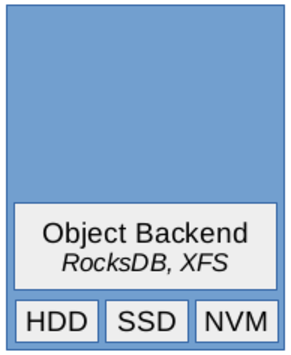
\includegraphics[width=1.0\linewidth]{figures/osd}
      \caption{OSD}
      \label{fig:osd}
  \end{subfigure}
  \caption{The Ceph cluster is composed of object storage devices (OSD) that
  provide access to objects on behalf of client requests. An OSD supports a
    wide variety of hardware and software configurations, as well as the
    transactional composition of object operations for defining
    application-level interfaces.}
\end{figure}

The object storage device (OSD), illustrated in Figure~\ref{fig:osd}, is the
building block of the RADOS cluster and is responsible for managing and
providing access to a set of
named objects. The configuration of an OSD is flexible, and commonly contains
a mix of commodity hardware such as HDD and SSD bulk storage, a multi-core
CPU, GBs of RAM, and one or two 10 Gb Ethernet links. Clients access object
data managed by an OSD by invoking native object operations exposed by the OSD
such as reading or writing bytes, as well as more complex operations like taking
snapshots or composing one or more native operations into compound procedures
that execute in a transactional context.

The native object operations in RADOS roughly fall into two categories based
on the type of data being accessed: key-value items, or bulk bytestream data.
The key-value interface operates as an isolated database associated with each
object, and the bytestream interface supports random byte-level access similar
to a standard file interface.  At a low-level each of these abstract I/O
interfaces map to hardware storage devices through a pluggable object backend
shown in Figure~\ref{fig:osd}. For instance, LevelDB or RocksDB may be used to
store key-value data, while the \emph{FileStore} implementation maps the
bytestream interface onto a local POSIX file system~\cite{leveldb,rocksdb} via
XFS or other supported file systems. Several backend implementations exist for
storing data in a range of targets such as HDD, SSD, as well as
Ethernet-attached disks, and NVMe devices using optimized access libraries.
%and in SMR disks using a specialized backend called BlueStore.

%Independent of the hardware or backends chosen, Ceph allows all
%object operations to be combined to create compound operations such as storing
%key-value metadata associated with a binary blob, allowing applications to
%build object interfaces that work even as Ceph software and hardware evolve.

\paragraph*{Object Classes}
While Ceph provides a wide variety of native object operations, it also
includes a facility referred to as \emph{object classes} that allow developers
to create application-specific object operations in the form of C++ shared
libraries dynamically loaded into the OSD process at runtime.  Object classes
can be used to implement basic data management tasks such as indexing
metadata, or used to perform complex operations such as data transformations
or filtering. Table~\ref{tab:objclass-cats} summarizes the range of object
classes maintained in the upstream Ceph project which support internal Ceph
subsystems as well as applications and services that run on top of Ceph.

\begin{table}[ht]
\centering
\begin{tabularx}{\columnwidth}{|X|l|l|l|}
\hline
Category & Specialization & Methods \\ \hline
\multirow{2}{*}{Locking} & Shared & \multirow{2}{*}{6} \\
                         & Exclusive & \\ \hline
\multirow{3}{*}{Logging} & Replica & 3 \\
                         & State & 4 \\
                         & Timestamped & 4 \\ \hline
Garbage Collection & Ref. Counting & 4 \\ \hline
\multirow{4}{*}{Metadata} & RBD & 37 \\
 & RGW & 27 \\
 & User & 5 \\
 & Version & 5 \\ \hline
\end{tabularx}
\caption{A variety of RADOS object storage interfaces exist that expose reusable
    interfaces to applications. The \emph{locking}, \emph{logging}, and
    \emph{GC} categories are generic, while high-level services like \emph{RBD} and
    \emph{RGW} implement application-specific metadata management interfaces.}
\label{tab:objclass-cats}
\end{table}

A critical step in the development of application-specific object interfaces
is deciding how to best make use of the native object interfaces. For instance
if an application stores an image in an object, it may also extract and store
EXIF metadata as key-value pairs in the object key-value database.  However,
depending on the application requirements it may be sufficient or offer a performance
advantage to store this metadata as a header within the bytestream. In the remainder
of this section we will explore the challenges associated with these design questions.

\subsection{Motivating Application: CORFU}

The primary motivating example we will use in this paper is the CORFU
distributed shared-log designed to provide high-performance serialization
across a set of flash storage devices~\cite{balakrishnan:nsdi12}. The
shared-log is a powerful abstraction useful when building distributed systems
and applications, but common implementations such as Paxos or Raft funnel I/O
through a single node limiting total throughput~\cite{lamport:tocs89}. The CORFU protocol addresses this limitation
by de-coupling log entry storage from log metadata management, making use of a
centralized, volatile, in-memory \emph{sequencer service} that assigns
positions to clients that are appending to the log. Since the sequencer is
centralized serialization is trivial, and the use of non-durable state allows
the sequencer service to operate at very high rates. The CORFU system has been
used to demonstrate a number of interesting services such as transactional
key-value and metadata services, replicated state machines, and an elastic
cloud-based database management system~\cite{balakrishnan:sosp13,bernstein:cidr11}.

Two aspects of CORFU make its design attractive in the context of the Ceph
storage system. First, CORFU assumes a cluster of flash devices because
log-centric systems tend to have a larger percentage of random reads making it
difficult to achieve high-performance with spinning disks. However, the speed
of the underlying storage does not affect correctness. Thus, in a
software-defined storage system such as Ceph a single implementation can
transparently take advantage of any software or hardware upgrades, and make use
of existing and future data management features such as tiering,
allowing users to freely choose between media types such as SSD, spinning
disks for archival storage, or emerging NVRAM technologies.

\paragraph*{CORFU and Storage Programmability}
The second property of CORFU relevant in the context of Ceph is the dependency
CORFU places on custom storage device interfaces used to guarantee
serialization during failure and reconfiguration. Each flash device in a CORFU
cluster exposes a 64-bit write-once address space consisting of the primary I/O
interfaces \emph{write(pos, data)} and \emph{read(pos)} for accessing log
entries, as well as \emph{fill(pos)} and \emph{trim(pos)} that invalidate and
reclaim log entries, respectively. All I/O operations in CORFU initiated by
clients are tagged with an \emph{epoch} value, and flash devices are expected
to reject client requests that contain an old epoch value. To facilitate
recovery or handle system reconfiguration in CORFU, the storage devices are
also required to support a \emph{seal(epoch)} command that stores the latest
epoch and returns the maximum position written to that device. The seal
interface is used following the failure of a sequencer to calculate the tail of
the log that the sequencer should use to repopulate its in-memory state.

While the authors of the CORFU paper describe prototype device interfaces
implemented as both host-based and FPGA-based solutions, RADOS \emph{directly} supports
the creation of logical storage devices through its object class feature
described previously in Section~\ref{sec:objclass}. Thus, by using
software-based object interfaces offered by RADOS flash devices in CORFU can be
replaced by software-defined storage offering significant flexibility and a
simplified design.

The implementation of a custom object class that satisfies the needs of an
application such as CORFU is often straightforward. However, as described in
Section~\ref{sec:objclass} there are a variety of native object I/O interfaces
available, and it is not always immediately clear how best to utilize these
interfaces.

\section{Physical Design Space}
\label{sec:pd}

As we have seen, Ceph provides a rich storage API and places few restrictions
on the structure of applications. Thus a primary concern when implementing an
object interface in Ceph is deciding how native interfaces are composed into
compound operations in order to implement the semantics of the target
interface. These types of decisions are commonly referred to as
physical design, and can affect performance and application flexibility.
As we will see the design space that developers must operate in is often
large, and its dynamic nature can lead to design decisions that become
obsolete and non-optimal.

\begin{figure}[t]
\centering
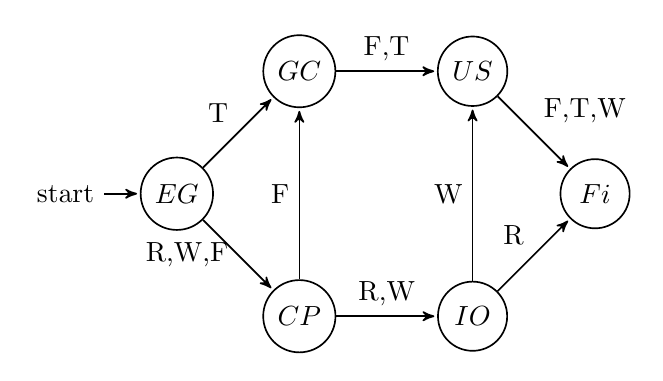
\begin{tikzpicture}[->,>=stealth',shorten >=1pt,auto,node distance=2.2cm,semithick]
%\tikzstyle{every state}=[fill=red,draw=none,text=white]

  \node[initial left,state] (A)              {$EG$};
  \node[state]         (B) [below right of=A] {$CP$};
  \node[state]         (D) [right of=B]       {$IO$};
  \node[state]         (C) [above right of=A] {$GC$};
  \node[state]         (E) [right of=C]       {$US$};
  \node[state]         (F) [below right of=E] {$Fi$};

  \path (A) edge        node [left] {R,W,F} (B)
            edge        node {T}     (C)
        (B) edge        node {F}     (C)
            edge        node {R,W}   (D)
        (C) edge        node {F,T}   (E)
        (D) edge        node {W}     (E)
            edge        node {R}     (F)
        (E) edge        node {F,T,W} (F);
\end{tikzpicture}
\caption{State transition diagram for read ($R$), write ($W$), fill ($F$), and
trim ($T$) CORFU operations. The states epoch guard ($EG$), check position ($CP$),
and update state ($US$) access metadata. The I/O performs a log entry read or
write, and garbage collection ($GC$) marks entries for reclamation.}
\label{fig:corfu-sm}
\end{figure}

To understand the developer process in the context of CORFU we have included the
state-machine diagram in Figure~\ref{fig:corfu-sm} showing the composition of
actions for each component of the CORFU interface which must be mapped onto
Ceph object classes. For instance, all operations begin by applying an
\emph{epoch guard} that ensures the request is tagged with an up-to-date epoch
value. The \emph{read} (R) and \emph{write} (W) operations both proceed by (1)
examining metadata associated with the target position, (2) performing I/O to
read or write the log entry, and in the case of a write, (3) updates metadata
for the target log position.

As an example, one valid design option is to store each log position in an
object with a name using a one-to-one mapping with the log entry position.
This would simplify the design of the \emph{write} interface because a small
amount of metadata stored as a header in the object could describe the state
of the log entry.  However, as we will see this choice of a physical design
can result in poor performance compared to other designs. In the remainder of
this section we will define the entire design space and use a set of targetted
benchmarks to arrive at a final design. Finally we will show that these design
decisions can lead to non-optimal decisions and suggest an automated approach
is desirable.

\subsection{Challenges}

The design space can be divided into three challenges: selecting a strategy
for log entry addressing, choosing a native I/O interface for storing log
entry content, and implementing efficient metadata management.

\begin{enumerate}
    \item {\bf Entry addressing.} We refer to the method by which a client
        locates a log entry in Ceph as entry addressing, and we consider two
        strategies. In a one-to-one (1:1) strategy each log entry is stored in
        a distinct object with a name derived from the associated log entry
        position. This is an attractive option because it is trivial for
        clients to locate a log entry given its position.  In contrast, an N:1
        strategy \emph{stripes} log entires across a smaller set of objects,
        but this adds complexity to both the client and the object interface which
        must multiplex a set of entries.

    \item {\bf Log entry storage.} Clients read and write binary data
        associated with each log entry, and these entries can be stored in the
        bytestream or in the key-value database associated with an object.
        Retrieval of log entry payloads should perform well for both large
        (e.g. database checkpoint) and small log entries.

    \item {\bf Metadata management.} The CORFU protocol defines the storage
        interface semantics, such as enforcing up-to-date epoch values and a
        write-once address space. The object interface constructed in Ceph must
        implement these semantics in software by storing metadata (e.g. the
        current epoch) and validating requests against this metadata (e.g. has
        the target position been written?). A key-value store is a natural
        location for this type of data, but metadata management adds overhead
        to each request and must be carefully designed.
\end{enumerate}

In the remainder of this section we will explore the full design space defined
by the cross product of these design challenges to arrive at a final design.

\subsection{Baseline Performance}

We begin the process of exploring the design space by exploiting the fact that
metadata management is a complexity and performance overhead that a full
implementation must incur beyond the costs of storing log entry data.
Therefore we first explore the design space by restricting the
space to log entry addressing and log entry storage (the \emph{I/O} action
shown in Figure~\ref{fig:corfu-sm}).  These two dimensions are
represented by the first two columns of Table~\ref{tab:pd-map} which describes
the entire design space. In the I/O column \emph{KV} corresponds to the
key-value interface, and the bytestream interface is represented by \emph{AP}
for an append strategy, and \emph{EX} for a strategy that writes to an
explicit bytestream offset (both described shortly).

\begin{table}[h]
\begin{tabular}{ | l | l | l | l | l |}
\hline
Map & I/O & Entry Size & Addressing & Metadata \\ \hline
\multirow{3}{*}{1:1} & KV  & Flex     & Ceph      & KV/BS \\ \cline{2-5}
                     & AP  & Flex     & Ceph/VFS  & KV/BS \\ \hline
\multirow{4}{*}{N:1} & KV  & Flex     & \multicolumn{2}{|c|}{KV/BS} \\ \cline{2-5}
                     & EX  & Fixed    & VFS       & KV/BS \\ \cline{2-5}
                     & AP  & Flex     & KV/BS     & KV/BS \\
\hline
\end{tabular}
\caption{The high-level design space of mapping CORFU log entry storage onto
the RADOS object storage system.}
\label{tab:pd-map}
\end{table}

\begin{figure*}[t]
	\centering
	\includegraphics[width=1.0\linewidth]{experiments/basic-cls-rand-read/jewel_v_firefly_v_es.png}
	\caption{The cluster-specific optimizations impact performance... a lot. This caption is quite terrible.
	\label{fig:jewel_v_firefly_v_es}}
\end{figure*}

The top row of Figure~\ref{fig:jewel_v_firefly_v_es} shows the expected
performance of different sized log appends without metadata management overhead
using each of the five strategies defined in Table~\ref{tab:pd-map}.  Starting
with Jewel and 4KB entry sizes, we see that both one-to-one strategies have
relatively poor performance. Jewel with 1KB entry sizes sees a 2.5\(\times\)
performance increase for the N:1 KV mapping. The large period of reduced
throughput for corresponds to the OSD splitting file system directories in
order to maintain a maximum directory size, and will occur in \emph{1:1, KV}
although the threshold number of objects is not reached in this example due to
the reduced overall throughput of the \emph{1:1, KV} strategy.

The second lesson that we can learn from the Jewel row of
Figure~\ref{fig:jewel_v_firefly_v_es} is that even when using an N:1 addressing
strategy, the key-value interface imposes a large overhead. This is unfortunate
because the key-value interface can provide a direct solution to addressing log
entries within an object.  Instead, what we find is that an N:1 addressing
strategy that stores log entries in the bytestream using either object appends
or writes to explicit offsets outperform all other strategies by a factor of
over 2\(\times\).

\begin{figure}[t]
      \centering
      \includegraphics[width=0.85\linewidth]{experiments/basic-cls-rand-read/output.read.60min.1k.png}
      \caption{The expected random read performance from a log with 1KB entries
      performs best on the same strategy that the write performance performs
      best on - the N:1 bystream append strategy.}
      \label{fig:vanilla_rd_jewel}
\end{figure}

The apparent performance tie between the strategies of appending to an object
and writing to explicit offsets can be broken by considering the flexibility
offered by each approach. The third column \emph{entry size} in
Table~\ref{tab:pd-map} shows if a particular strategy supports storage of
entries with dynamic sizes, or if entries must be restricted to a fixed size.
Notably the strategy that stores log entries at explicit object offsets is
limited in this regard because each log entry is effectively pre-mapped into
the storage system. This leaves the clear winner: an N:1 strategy that appends
log entries to objects provides flexibility and the best write performance in
this particular configuration.  This result is corroborated by considering the
read performance for each strategy as well. Figure~\ref{fig:vanilla_rd_jewel}
shows the expected random read performance from a log containing 1K entries in
which an addressing strategy that stores log entries in the bytestream has the
best performance.

\subsection{Metadata Management}

The previous results show that storing log entries in the bytestream has the
potential to provide the best overall performance, but by design, those
results do not contain the real-world overheads introduced by metadata
management such as validating that requests are tagged with an up-to-date
epoch value. Having only focused on entry I/O costs, in this section we
consider the overhead of the remaining actions shown in
Figure~\ref{fig:corfu-sm}.

\begin{enumerate}
    \item {\bf Epoch guard.} Each client request must be validated against the
        current epoch. This singleton value in infrequently updated, but the
        cost of accessing the value must be incurred for every request.

    \item {\bf Per-entry metadata.} Unlike the singleton epoch value, metadata
        associated with each log position must be read, and optionally updated
        for every request. For instance the \emph{fill} operation must ensure
        that it is not applied to a log position that has already been
        written. When an operation that changes a log position is successful
        (i.e. \emph{write}, \emph{fill}, \emph{trim}) the per-entry metadata
        must also be updated to reflect the change. While the size of the
        per-entry metadata is small, it is accessed for every operation and a
        single object may manage a large number of entries.
\end{enumerate}

The design space for managing metadata can be large depending on the
application. In many cases this space is significantly reduced when the
key-value interface is used because it handles a large portion of common data
management challenges such as indexing. On the other hand, we have seen that
the bytestream can be used to achieve much higher performance when used in
lieu of the key-value database, but leaves the design space wide open.

\begin{figure}[t]
	\centering
	\includegraphics[width=0.85\linewidth]{experiments/basic-cls-overhead/output.1024.soft.reset.png}	
	\caption{1hr,1k,cls\_wr,jewel: this graph shows the overhead of class}
	\label{fig:cls_wr_jewel}
\end{figure}

We consider two high-level design prototypes in this paper based on both the
key-value and bytestream interfaces. The summary of performance of these
designs is shown in Figure~\ref{fig:cls_wr_jewel} where we begin by
highlighting two baseline throughputs labeled \emph{librados} and
\emph{cls\_null} that correspond to the baseline append throughput described
in the previous section, and the append throughput achieved with \emph{object
class} overhead included. We will discuss the performance of our two prototype
designs relative to the base cost of using \emph{object class} facility.

The first design is based on the key-value interface. In this design the epoch
value is stored under a fixed key, and the metadata associated with each log
entry is stored under a key derived from the log position. The expected throughput of
this design is shown in Figure~\ref{fig:cls_wr_jewel} and labeled as
\emph{cls\_full\_omap}. This result shows us that even for very small values
the cost of managing data in the key-value store introduces significant
overhead. In contrast, the unstructured bytestream interface imposes little
to no restriction on how it is used.

An obvious choice for encoding the singleton epoch value in the bytestream is
to position it at a fixed offset such as in a header. A method for indexing
entry metadata is far less obvious. Solutions span a wide design spectrum and
include approaches such as encoding a search tree into the bytestream, or
exploiting the regularity log addressing and storing a dense array that can be
efficiently indexed. While there is clearly a wide variety of approaches, we
have chosen to examine the overhead incurred by an hypothetical best-case
design in which per-entry metadata can be accessed with a single I/O. The I/O
overhead of the test includes (1) read epoch value from a fixed header
location, (2) read the per-entry metadata, and in the case of an update (3)
write the updated per-entry metadata. The expected throughput from such a
design is shown in Figure~\ref{fig:cls_wr_jewel} labeled as
\emph{cls\_full\_hdr} and performs with roughly a 6\% overhead.

Application-level designs also contribute to an expanded design space.  In the
N:1 design of mapping CORFU onto Ceph the potential amount of I/O parallelism
is controlled by the value N, however if this value becomes too large there may
be no benefit or performance could suffer from reduced data locality. Other
aspects of application-level design are even more flexible. A wide variety of
data structures could be serialized into the byte stream to handle metadata
management tasks, but selecting a single external index that performs well
across workloads and hardware may not be possible.

\subsection{Cluster-Specific Optimizations}

In this section we have demonstrated that a design based on an N:1 addressing
scheme that stores both log entries and metadata in the bytestream can provide
the best overall performance, and it does so by a large margin. However, this
process of design we have outlined may not yield such clear cut results when
applied in a different context. To illustrate these contexts, we describe the
software, system tunable, and hardware parameters that affect the performance
of our CORFU implementation. The complexity and breadth of our parameter sweep,
and the fact that our state space grew so large, motivates brados in section 4.

\subsubsection{Software Parameters}

Ceph releases stable versions every year (Oct/Nov) and LTS versions every 3-4
months~\cite{website:ceph-releases}. The head of the master branch moves
quickly because there are over 400 contributors and an active mailing list.
Over the past calendar year, there were between 70 and 260 commits per
week~\cite{website:ceph-github}. 

\textbf{Ceph Versions}: to show the evolution of Ceph's performance and
behavior, we ran the same benchmark, which measures append throughput, with the
same configurations, hardware, and tunables on 2 versions of Ceph: Jewel (April
2016) - the newest stable release and Firefly (May 2014) - a long term support
version that introduced cache tiering and erasure coding. The Jewel row of 
Figure~\ref{fig:jewel_v_firefly_v_es} shows that the size of the log entries
has a clear impact on performance but the Firefly release shows no such trend.
The fact that the appends per second are an order of magnitude slower on
Firefly indicates that the the benchmark is bottlenecked by the Ceph software
instead of the external log implementation. 

The bytestream interface outperforms the key-value interface by 12\%, compared
to over 100\% in the newer version of Ceph. Qualitatively, given the reduced
overall throughput achieved in the older version, some developers may find that
incurring the overhead of using the key-value interface is an easy decision
given the reduced complexity of the design space for metadata management. If
this choice had been made, then a future system upgrade could drop a
significant number of iops on the floor.

\textbf{Ceph Features}: to show the affect of cutting-edge Ceph features, we
now show results for BlueStore~\cite{weil:vault2016-bluestore}. BlueStore is a
replacement for the FileStore file system in the OSD (traditionally XFS).
FileStore has performance problems with transactions and enumerations; namely
the journal needed to assure atomicity incurs double writes and the file system
metadata model makes object listings slow, respectively. BlueStore stores data
directly on a block device and the metadata in RocksDB, which is provided by a
minimalistic, non-POSIX C++ filesystem. This model adheres to the overall
software defined storage strategy of Ceph because it gives the administrator
the flexiblity to store the 3 componenets of BlueStore (e.g., data, RocksDB
database, and RocksDB write-ahead log) on any partition on any device in the
OSD. 

\textbf{Takeway}: choosing the best implementations is dependent on both the
timing of the developemnt (Ceph Version) and the expertise of the administrator
(Ceph Features). Different versions and features of Ceph may lead the
administrator to choose a suboptimal implementation for the system's next
upgrade. The software parameters must be accounted for and benchmarked when
making design decisions.

\subsubsection{System Tunables}

The most recent version of Ceph (v10.2.0-1281-g1f03205) has 994 tunable
parameters\footnote{This number comes from \texttt{src/common/config\_opts.h}
with debug options filtered out.}, where 195 of them pertain to the OSD itself
and 95 of them focus on the OSD back end file system (i.e. its
\texttt{filestore}). Ceph also has tunables for the subystems it uses, like
LevelDB (10 tunables), RocksDB (5 tunables), its own key-value stores (5
tunables), its object cache (6 tunables), its journals (24 tunables), and its
other optional filestores like BlueStore (49 tunables).

This many domain-specific tunables makes it almost impossible to come up with
the best set of tunables, although auto-tuning like the work done
in~\cite{behzad:sc2013-autotuning} could go a long way. Regardless of the
technique that we use, it is clear the the number of tunables increases the
physical design parameters to an unwieldy stae space size.

\textbf{Takeaway}: the number and complexity of Ceph's tunables make
brute-force parameter selection impossible.

\subsubsection{Hardware Parameters}

\begin{figure}[t]
	\centering
	\includegraphics[width=1.0\linewidth]{experiments/basic-cls-rand-read/jewel-hdd-128b.png}
	\caption{shows that with a HDD, it don't matter if you choose omap!!!!!}
	\label{fig:jewel-hdd-128b}
\end{figure}

Ceph is designed to run on a wide variety of commodity hardware as well as new
NVMe devices, all of which their own set of characteristics and tunables (e.g.,
the IO operation scheduler type). In our experiments, we tested SSD, HDDs, NVMe
devices and discovered a wide range of behaviors and performance profiles.
Figure~\ref{fig:jewel-hdd-128b}, which shows the write performance of 128 by
log entries using Jewel and a single HDD, shows an especially tricky situation
for a developer. 

In that figure, the performance is 10\(\times\) slower than its SSD counterpart
but performance of the N:1 bystestream implementation is almost identical to
the N:1 KV implementation (within 1\% mean throughput). Regardless of the true
bottleneck, it is clear that choosing the N:1 KV implementation is the better
choice because of the simple implementation and the minimal performance
degradation.

\textbf{Takeaway}: choosing the best implementations is dependent on hardware.
Something as common as an upgrade from HDD to SSD may nullify the benefits of a
certain implementation. 

\subsection{Discussion}

This physical design process, of first thinking about the design trade-offs and
then doing parameters sweeps, is insufficient when general-purpose systems. Had
we built ZLog from the ground up (like CORFU) the story might be different but
to deal wtih the large state space we need a way to automatically and
autonomically decide which parameters to choose. 

Next we present a declarative programming model that seeks to solve the issue
of selecting an optimal mapping between application requirements and object
class implementation.

\section{The Brados Programming Model}

As Ceph continues to develop into a target for building distributed services
and application, it is important to not restrict use to developers seasoned
in distributed programming and those with knowledge of intricacies of the Ceph
performance model. To this end we present Brados, a declarative language with
relational semantics for defining the behavior of RADOS object interfaces.
Brados uses a simple declarative data model and can reduce the learning curve
for new users, and allows existing developers to increase productivity by
writing less code that is more portable.

The Brados language corresponds to a subset of the Bloom language, and models the
storage system state uniformly as a collection of
relations~\cite{alvaro:cidr11}. The composition of a collection of existing
interfaces is then expressed as a collection of high-level \emph{queries} that
describe how a stream of requests (API calls) are filtered, transformed and
combined with existing state to define streams of outputs (API call returns as
well as updates to system state).  Separating the relational semantics of such
compositions from details of their physical implementations introduces a
number of degrees of freedom, similar to the ``data independence'' offered by
database query languages.  The choice of access methods (for example, whether
to use a bytestream interface or a key/value store), storage decide
classes(e.g., whether to use HDDs or SDDs), physical layout details (e.g. a
1:1 or 1:N mapping) and execution plans (e.g.  operator ordering) can be
postponed to execution time.  The optimal choices for these physical design
details are likely to change much more often than the logical specification,
freeing the interface designer from the need to rewrite systems and device and
interface characteristics change.  

\subsection{Basics}

\subsection{The CORFU Log Interface}

\begin{lstlisting}[caption={State Declaration}, label=lst:state]
state do
  table :epoch, [:epoch]
  table :log, [:pos] => [:state, :data]

  interface input, :op,
    [:type, :pos, :epoch] => [:data]

  interface output, :ret,
    [:type, :pos, :epoch] => [:retval]

  scratch :write_op, op.schema
  scratch :read_op,  op.schema
  scratch :trim_op,  op.schema
  scratch :fill_op,  op.schema
  scratch :seal_op,  op.schema

  # op did or did not pass the epoch guard
  scratch :valid_op,   op.schema
  scratch :invalid_op, op.schema

  # op's position was or was not found in the log
  scratch :found_op,    op.schema
  scratch :notfound_op, op.schema
end
\end{lstlisting}

\begin{lstlisting}[caption={Setup}, label=lst:setup]
bloom do
  # op's position found in log
  found_op <= (valid_op * log).lefts(pos => pos)
  notfound_op <= valid_op.notin(found_op)

  # demux on operation type
  write_op <= valid_op {|o| o if o.type == 'write'}
  read_op  <= valid_op {|o| o if o.type == 'read'}
  fill_op  <= valid_op {|o| o if o.type == 'fill'}
  trim_op  <= valid_op {|o| o if o.type == 'trim'}
  seal_op  <= valid_op {|o| o if o.type == 'seal'}
end
\end{lstlisting}

Listing~\ref{lst:eg} shows the epoch guard that is applied to all operations.
The guard rejects requests that are tagged with old epoch values, ensuring that
a client generating a request has an up-to-date view of the system.  First the
\texttt{invalid\_op} collection is defined to include the current operation if
its epoch value is no larger than the stored epoch value. Next the
\texttt{valid\_op} collection is defined to be the inverse of
\texttt{invalid\_op} and is a helper used to refine other operations later in
the dataflow. Finally we handle the case for all operations tagged with an
out-of-date epoch by merging the \texttt{invalid\_op} set into the output
\texttt{ret} collection.

\begin{lstlisting}[caption={Epoch Guard}, label=lst:eg]
bloom :epoch_guard do
  invalid_op <= (op * epoch).pairs{|o,e|
    o.epoch <= e.epoch}
  valid_op <= op.notin(invalid_op)
  ret <= invalid_op{|o|
    [o.type, o.pos, o.epoch, 'stale']}
end
\end{lstlisting}

The process of sealing an object requires installing a new epoch value and
returning the current maximum position written. Listing~\ref{lst:seal} 
implements the seal interface by first removing the current epoch value and
replacing it with the epoch value contained in the operation. Next an aggregate
is computed over the log to find the maximum position written, and this value
is returned.

\begin{lstlisting}[caption={Seal}, label=lst:seal]
bloom :seal do
  epoch <- (seal_op * epoch).rights
  epoch <+ seal_op { |o| [o.epoch] }
  temp :maxpos <= log.group([], max(pos))
  ret <= (seal_op * maxpos).pairs do |o, m|
    [o.type, nil, o.epoch, m.content]
  end
end
\end{lstlisting}

Trimming a log entry always succeeds. In Listing~\ref{lst:trim} The
\texttt{<+-} operator simulatenously removes the log entry with the given 
position and replaces it with an entry with its state set to \emph{trimmed}.

\begin{lstlisting}[caption={Trim}, label=lst:trim]
bloom :trim do
  log <+- trim_op{|o| [o.pos, 'trimmed']}
  ret <=  trim_op{|o|
    [o.type, o.pos, o.epoch, 'ok']}
end
\end{lstlisting}

The write and fill interfaces are implemented similarily, and are show in
Listing~\ref{lst:write} and Listing~\ref{lst:fill}, respectively.  A valid
write collection is created if the operation position is not found in the log.
A valid write operation is then merged into log, otherwise a read only error is
returend indicating that the log position was already written to.
The fill operation is identical except a the fill state is set on the log entry.

\begin{lstlisting}[caption={Write}, label=lst:write]
bloom :write do
  temp :valid_write <= write_op.notin(found_op)
  log <+ valid_write{ |o| [o.pos, 'valid', o.data]}
  ret <= valid_write{ |o|
    [o.type, o.pos, o.epoch, 'ok'] }
  ret <= write_op.notin(valid_write) {|o|
    [o.type, o.pos, o.epoch, 'read-only'] }
end
\end{lstlisting}

\begin{lstlisting}[caption={Fill}, label=lst:fill]
bloom :fill do
  temp :valid_fill <= fill_op.notin(found_op)
  log <+ valid_fill { |o| [o.pos, 'fill'] }
  ret <= valid_fill { |o|
    [o.type, o.pos, o.epoch, 'ok'] }
  ret <= fill_op.notin(valid_fill) { |o|
    [o.type, o.pos, o.epoch, 'read-only'] }
end
\end{lstlisting}

The read interface is shown in Listing~\ref{lst:read}, and structured similar
to the write interface. First we create a collection containing a valid read
operation that is in the log and does not have the filled or trimmed state set.
The data is returend in the case of a valid read op, otherwise an error is
returend through the output interface.

\begin{lstlisting}[caption={Read}, label=lst:read]
bloom :read do
  temp :ok_read <= (read_op * log).pairs(pos => pos) { |o, l|
    [o.type, o.pos, o.epoch, l.data] unless
      ['filled', 'trimmed'].include?(l.state) }
  ret <= ok_read { |e|
    [e.type, e.pos, e.epoch, e.data] }
  ret <= read_op.notin(ok_read, type=>type) do |o|
    [o.type, o.pos, o.epoch, 'invalid']
  end
end
\end{lstlisting}

Amazingly these few code snippets express the semantics of the entire storage
device interface requirements in CORFU. For reference the ZLog implementation
of the CORFU storage interface in C++ comprises nearly 700 lines of code and
was designed to store log entries and metadata in the key-value interface,
thus requiring a lengthy rewrite to realize the performance advantage
available by using the bytestream interface, as was highlighted in
Section~\ref{sec:pd}. Furthermore, the complexity introduced by using the
bytestream interface would grow the amount of code written in the optimized
version.

But beyond the convience of writing less code, it is far easier for the
programmer writing an interface such as CORFU to convinence herself of the
correctness of the high-level details of the implementation without being
distracted by issues related to physical design or the many other gotchas that
one must deal with when writing low-level systems software.

\subsection{Optimization}

Choosing implementation details
  - the refcount example is good. small data kept in ceph object bytestream
until it becomes large then use omap.

  - could use the dataflow graph to do interesting things like understand how
  to do prefecting of things like keys or data that are often only known at
  execution time

\subsection{Other Interfaces}

As we have seen the subset of Bloom used in Brados is powerful enough to
express the semantics of the CORFU storage interface. We briefly sketch the
implementation of an additional interface found in Ceph that used by the
S3-compatible RADOS-Gateway service to perform object reference counting.

The reference count implementation that we describe does not use a typical
counter, but rather uses a tag-based interface in which each \emph{reference}
to an object is identified by a application-level tag. Each tag represents
one or more references allowing an idempotent property useful for application
that may replay reference count operations out of order. Otherwise the
semantics are straightforward: clients record references to an object, and
when the number of references drop to zero the object is removed.

The reference implementation in Ceph is 300 LOC written in C++. The version
written in Brados is shown in Listing~\ref{lst:rc}.

 Unlike the CORFU interface
that took advantage of a mapping between backend storage and collections, the
reference counting interface requires access to RADOS runtime facilities that
allow objects to be removed. This is modeled in Brados using the Bloom
\emph{channel} abstraction that is used to transmit facts between entities in
the system; we effectively send a message to the runtime with our removal
request.

\begin{lstlisting}[caption={Reference counting interface}, label=lst:rc]
state do
  table :refs, [:tag]
  channel :remove_chn
  interface input, :get_op, [:tag]
  interface input, :put_op, [:tag]
  interface output, :ret, [:status]
end

bloom :get do
  refs <= get_op
  ret  <= get_op{|op| ['ok']}
end

bloom :put do
  temp :found <= (put_op * refs).matches
  refs <- found
  ret <= put_op{|op| ['ok']}

  temp :remove <= found.notin(refs)	
  remove_chn <~ remove
end
\end{lstlisting}

\section{Evaluation}

\section{Related Work}

{\bf Active storage.}
There is a wide variety of work related \emph{active storage} that seeks to
increase performance and reduce data movement by exploiting remote storage
resources. This concept has been applied in the context of on-disk
controllers and object-based storage
(T10)~\cite{riedel:vldb98,du:nwesp05,xie:msst11}.  Solutions to safety
concerns have examined using managed lanuages, sandbox technologies, as well
as restricting extension installation to
vendors~\cite{john:hiperio08,xie:msst11,runde:msst12}.

Techniques for remote storage processing have been applied in
application-specific domains for database and file system acceleration, as
well as in remote data filtering in cloud-based storage
environments~\cite{uysal:hpca00,chiu:iccs03,lim:msst08,gkantsidis:nsdi13}
Others have collected and used statistics to optimize the location of
computation in general workloads as well as database systems
~\cite{chen:cluster12,chen:icpp12,qiao:icde08}.

Most closely related to our work are efforts that consider specific
programming models in the context of active storage such as a stream-based
model~\cite{acharya:asplos98}, a model that assisted in optmiizing balancing
computation~\cite{wickremesinghe:hpdc022}, and optimization that took
advantage of read-only data to reorder operations~\cite{huston:fast04}.
While our goals are similar to previous work, we start with a declarative
language that will enable us to apply optimization techniques beyond
the limited domain-specific optimizations found in previous work.

{\bf Declarative Specifications.}
Declarative interfaces have been used for specifying distributed analytic 
tasks~\cite{olston_pig_2008,thusoo_hive_2010}, information 
extraction~\cite{shen_declarative_2007} and distributed 
systems~\cite{conway_logic_2012,bauer_legion_2014}. The use of declarative 
specifications has also been explored in other contexts such as cloud recovery 
testing~\cite{gunawi_fate_2011}, bug reproduction~\cite{li_reprolite_2014} and 
cloud resource orchestration~\cite{liu_declarative_2011}.

\section{Conclusion and Future Work}

Much work remains to be done.  While we demonstrated some of the immediate
benefits of separating logical and physical specifications of component
compositions, the ``dream’’ of data independence is to take the physical
design question completely off the table for programmers.  We are currently
exploring both cost-based optimizers and autotuners to automate the selection
of a high performance physical design consistent with a given logical
specification.  

The database literature on materialized view maintenance and selection can be
brought to bear in the context of programmable storage as well.  Recall the
sequencer logic of Corfu described in Section XX.  The Bloom specification
(Figure YY) simply states that the current value of the sequencer is the
result of evaluating an aggregate query over the log relation.  This means
that the system may choose any strategy to maintain a sequence value that is
consistent with this constraint.  The physical design decision to store and
update a memory-resident sequence value rather re-computing the maximal value
at each request is a view materialization decision that could similarly be
made by a compile-time optimizer.

The future of programmable storage is likely to witness a further
decomposition of services to allow greater flexibility in customizing
deployments.  More than likely, not all of these services will assume or
provide strongly-consistent operations by default.  Instead, programmers will
have the flexibility (and burden!) of trading off between performance (offered
by weakly consistent subsystems) and programmability.  Languages such as
Bloom---which provide static analyses to determine when loosely-ordered
operations nevertheless produce consistent outcomes---will become increasingly
relevant in this domain.

%Include performance management topic in future work.

\bibliography{paper}
\bibliographystyle{plain}

\end{document}
